% ch12-ml.tex -- Generative models
\chapter{Generative models}
\label{ch:gen}

Everything so far learned a conditional: $p(y \mid \mathbf x)$ --- a
label given pixels, a price given rooms. This chapter flips the arrow.
A \emph{generative model}\index{generative model} learns $p(\mathbf x)$
itself --- the distribution of the data --- which is the object you must
hold before you can \emph{sample} new digits, detect weird ones, or say
how surprising an observation is. The catch is that $p(\mathbf x)$ is
enormously harder to fit than $p(y\mid\mathbf x)$: a classifier only
needs the boundary; a generative model needs the whole map. We build
three honest representatives of the three great families --- an
autoregressive baseline on pixels, a variational autoencoder with a
real ELBO, a diffusion sampler on a spiral --- plus a tiny GAN that
collapses on camera so you can see the failure, not just read about it.
Each section ends the same way: \emph{sample, then interrogate} ---
because the whole discipline of generative modelling is that a pretty
sample proves almost nothing.

% from-zero:begin
\begin{rulebox}[Before you start]
Chapters~7--11 and \textbf{Book~3, Chapters~12 and~15} (probability, KL divergence). \emph{Recap:} a generative model learns $p(\mathbf x)$, the distribution of the data itself, so that it can produce new samples.
\end{rulebox}
\begin{wins}[After this chapter you can]
\begin{itemize}
\item say how generative and discriminative models differ;
\item factor a distribution autoregressively;
\item explain the VAE objective, GAN training, and diffusion at the level of one equation each;
\item say why evaluating generative models is hard.
\end{itemize}
\end{wins}
\begin{principle}[How to think about this]
Instead of predicting a label, a generative model learns to create. Each family (autoregressive, VAE, GAN, diffusion) is a different answer to one question: how do I turn simple randomness into realistic data? Judge a model by what it makes, and be sceptical of any single number that claims to measure quality.
\end{principle}
% from-zero:end

\section{Generative vs discriminative: $p(\mathbf x)$ vs $p(y\mid\mathbf x)$}
\label{sec:gvd}

A discriminative model\index{discriminative model} partitions space:
it can be brilliant at $p(y\mid\mathbf x)$ while knowing nothing about
what data looks like. A generative model must answer ``how much does
this point look like training data?'' --- a density, a sampler, or
both. That extra requirement buys three things a classifier cannot do:
\textbf{sample} new examples (data augmentation, simulation),
\textbf{score} anomalies (low $p(\mathbf x)$ $\approx$ outlier), and
\textbf{impute} missing pieces (condition on the observed part).

\begin{figure}[htbp]
\centering
\begin{tikzpicture}[scale=0.9,font=\small]
% left: discriminative
\draw[thick] (-0.4,-0.4) rectangle (4.6,3.4);
\node[anchor=north] at (2.1,-0.55) {discriminative: the boundary};
\draw[thick,accent] (0.4,0.4) .. controls (1.6,1.8) and (2.6,0.9) .. (4.2,2.9);
\foreach \x/\y in {0.6/2.6,1.2/3.0,0.9/2.0,1.7/2.6,2.0/2.2,2.9/2.6}
  \node[slate] at (\x,\y) {$\times$};
\foreach \x/\y in {0.7/0.6,1.5/0.5,2.2/0.9,3.3/0.7,3.7/1.5,2.6/1.1}
  \node at (\x,\y) {$\circ$};
\node[font=\scriptsize,slate] at (1.0,3.15) {$p(y{=}+{\mid}\mathbf x)$ only};
% right: generative
\draw[thick] (5.6,-0.4) rectangle (10.6,3.4);
\node[anchor=north] at (8.1,-0.55) {generative: the density};
\draw[thick,accentsoft] (7.0,2.4) ellipse (1.05 and 0.65);
\draw[thick,accentsoft!60] (7.0,2.4) ellipse (1.7 and 1.0);
\draw[thick,amberbg] (8.9,0.8) ellipse (0.95 and 0.55);
\draw[thick,amberbg!60] (8.9,0.8) ellipse (1.45 and 0.85);
\foreach \x/\y in {6.4/2.5,7.2/2.7,7.6/2.2,6.8/2.1,7.1/2.6}
  \node[slate] at (\x,\y) {$\times$};
\foreach \x/\y in {8.5/0.9,9.3/0.7,9.0/1.1,8.8/0.5,9.4/1.0}
  \node at (\x,\y) {$\circ$};
\node[font=\scriptsize,slate] at (8.1,3.15) {$p(\mathbf x)$ --- where data lives};
\end{tikzpicture}
\caption{Two questions on the same data. Left: the discriminative
answer --- one boundary, everything else ignored. Right: the
generative answer --- where each class's mass actually sits, so a
point far from \emph{both} blobs can be called unlikely, not just
classified.}
\label{fig:gvd}
\end{figure}

The price is honesty about evaluation. A classifier's accuracy is one
number everyone agrees on; a generative model's quality splits into
\emph{likelihood} (does it score held-out data high?), \emph{sample
fidelity} (do samples look real?), and \emph{coverage} (does it make
\emph{all} the kinds of things, or only the easy kinds?) --- and these
three routinely disagree, as \S\ref{sec:evalgen} will show on our own
outputs.

\section{Autoregressive models: the chain factorisation}
\label{sec:ar}

The oldest working idea: factorise the joint by the chain
rule\index{autoregressive model}
\[
p(\mathbf x) = \prod_{d=1}^{D} p(x_d \mid \mathbf x_{<d}),
\]
and learn each conditional separately. Chapters 10--11 were already
this: a char-LM is a chain factorisation where each conditional is a
neural net over the past. On an $8{\times}8$ digit the ``past'' is just
the previous pixels; even a one-pixel context buys real structure.

\lstinputlisting[language=Python,caption={\texttt{code/ch12/sample\_compare.py}: two generative baselines on binarised \texttt{digits} --- a pixel-\emph{independent} model and an autoregressive one conditioned on the previous pixel --- with held-out NLL/pixel and sampled grids.},label=lst:samples]{code/ch12/sample_compare.py}

\lstinputlisting[numbers=none]{code/ch12/sample_compare.out.txt}

\begin{example}[WE 12.1 --- Context is worth 0.02 nats per pixel]
\label{ex:ar}
Read the listing's numbers the ch3 way: per-pixel negative
log-likelihood on 397 held-out images is $0.3943$ for the
pixel-independent model and $0.3740$ for the one conditioned on the
previous pixel. That $\Delta = 0.0203$ nats/pixel compounds across
64 pixels to $e^{0.0203 \times 64} \approx e^{1.30} \approx 3.7\times$:
a held-out digit is $3.7\times$ more likely under the model that
\emph{looks at its context} --- the entire generative-modelling
argument in one subtraction. And it is the same argument as ch10's
trigram-vs-LSTM table, one level down: each extra unit of context buys
a small, honest, measurable slice of likelihood.
\end{example}

\begin{figure}[htbp]
\centering
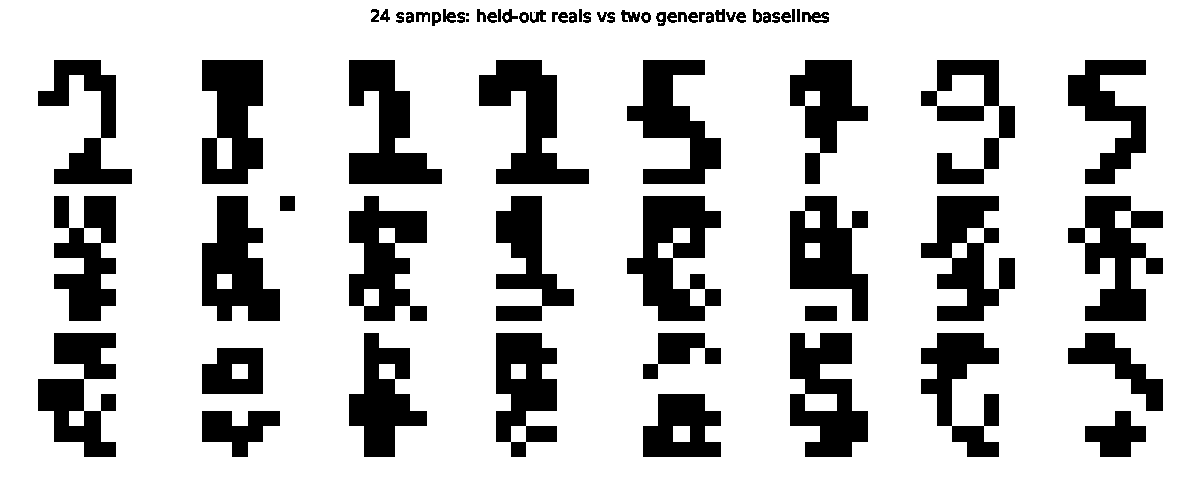
\includegraphics[width=0.94\linewidth]{figures/ch12/samples.pdf}
\caption{The two baselines, sampled
(\texttt{code/ch12/sample\_compare.py}): real digits (top),
independent-pixel samples --- salt-and-pepper noise with the right
marginals (middle), prev-pixel-AR samples --- recognisably digit-like
because each pixel sees its left neighbour (bottom). The middle row is
the lesson: matching every marginal independently still misses the
\emph{joint}.}
\label{fig:samples}
\end{figure}

Autoregression scales to the state of the art --- PixelCNN, GPT ---
because chain factorisation is \emph{exact}, trainable by plain
maximum likelihood, and each conditional is a supervised problem we
already know how to fit. The costs are also inherited: sampling is
sequential (pixel 64 cannot be drawn until pixels 1--63 exist), and a
mistake made early compounds --- the teacher-forcing gap of ch10,
pixel edition.

\section{Latent-variable models and the VAE}
\label{sec:vae}

If modelling every pixel explicitly is expensive, postulate a small
\emph{latent}\index{latent variable} $\mathbf z$ that generates
$\mathbf x$: $p(\mathbf x) = \int p(\mathbf x \mid \mathbf z)\,
p(\mathbf z)\,d\mathbf z$. The integral is intractable, so the
\textbf{VAE}\index{VAE}~\cite{kingma2013} maximises a tractable lower
bound instead --- the ELBO\index{ELBO}:
\[
\log p(\mathbf x) \;\geq\; \underbrace{\mathbb E_{q(\mathbf z\mid
\mathbf x)}\big[\log p(\mathbf x\mid\mathbf z)\big]}_{\text{reconstruction}}
\;-\; \underbrace{\mathrm{KL}\!\big(q(\mathbf z\mid\mathbf x)
\,\|\, p(\mathbf z)\big)}_{\text{stay near the prior}}.
\]
An \emph{encoder} net produces $q(\mathbf z\mid\mathbf x) = \mathcal
N(\boldsymbol\mu, \mathrm{diag}\,\boldsymbol\sigma^2)$; a
\emph{decoder} reconstructs; the KL term pulls the posteriors toward
a standard normal prior so that \emph{sampling} works --- draw
$\mathbf z \sim \mathcal N(0,I)$, decode, get a plausible $\mathbf x$.
The trick that makes it differentiable is the
\emph{reparameterisation}\index{reparameterisation trick}: write
$\mathbf z = \boldsymbol\mu + \boldsymbol\sigma \odot
\boldsymbol\epsilon$ with $\boldsymbol\epsilon \sim \mathcal N(0,I)$
and the gradient flows through $\boldsymbol\mu,\boldsymbol\sigma$
while the noise stays outside the graph.

\begin{figure}[htbp]
\centering
\begin{tikzpicture}[font=\small,
  blk/.style={draw,minimum width=16mm,minimum height=8mm},
  arr/.style={->,thick}]
\node[blk,fill=accentsoft] (x) {$\mathbf x$};
\node[blk,fill=accentsoft,right=9mm of x] (enc) {encoder};
\node[blk,fill=amberbg,right=9mm of enc] (q) {$\boldsymbol\mu,\boldsymbol\sigma$};
\node[blk,right=9mm of q] (z) {$\mathbf z$};
\node[blk,fill=accentsoft,right=9mm of z] (dec) {decoder};
\node[blk,fill=accentsoft,right=9mm of dec] (xh) {$\hat{\mathbf x}$};
\draw[arr] (x)--(enc); \draw[arr] (enc)--(q);
\draw[arr] (q)-- node[above]{\scriptsize $+\boldsymbol\sigma\odot\epsilon$} (z);
\draw[arr] (z)--(dec); \draw[arr] (dec)--(xh);
\node[below=4mm of z,font=\scriptsize] {$\mathbf z\sim\mathcal N(0,I)$ at sampling time};
\draw[arr,dashed,slate] (xh.north) .. controls (4.2,1.5) and (2.2,1.5) .. node[above,slate,font=\scriptsize]{reconstruction loss} (x.north -| enc);
\node[below=4mm of q,font=\scriptsize,slate] {KL$(q\,\|\,p)$ to $\mathcal N(0,I)$};
\end{tikzpicture}
\caption{The VAE loop. Left to right: data in, posterior out, sample
via reparameterisation, decode, score the reconstruction. The KL
term --- the dashed pressure toward the prior --- is what turns a
training-time encoder into a sampling-time generator.}
\label{fig:vaearch}
\end{figure}

\lstinputlisting[language=Python,caption={\texttt{code/ch12/vae\_torch.py}: a small VAE on \texttt{digits} --- encoder $64{\to}128{\to}(\mu,\mathrm{logvar},z_8)$, decoder $z_8{\to}128{\to}64$ --- with the ELBO broken into its two terms and a nearest-neighbour honesty probe at the end.},label=lst:vae]{code/ch12/vae_torch.py}

\lstinputlisting[numbers=none]{code/ch12/vae_torch.out.txt}

\begin{example}[WE 12.2 --- The two terms fight, and both lose a little]
\label{ex:elbo}
Watch the printed components, not just the total: reconstruction
(BCE) falls $44.3 \to 20.5$ while KL \emph{rises} $0.1 \to 3.7$. That
is not a bug --- it is the deal. Early on the encoder shrugs ($q
\approx$ prior, KL $\approx 0$, terrible reconstructions); as the
decoder improves, the encoder dares to put information in $\mathbf z$,
which costs KL. The ELBO's final $24.2 = 20.5 + 3.7$ is the negotiated
settlement. If KL had stayed $0$ the model would be an ordinary
autoencoder --- good reconstructions, useless samples, because the
posterior would be a scatter of spikes no $\mathcal N(0,I)$ draw could
hit.
\end{example}

\begin{figure}[htbp]
\centering
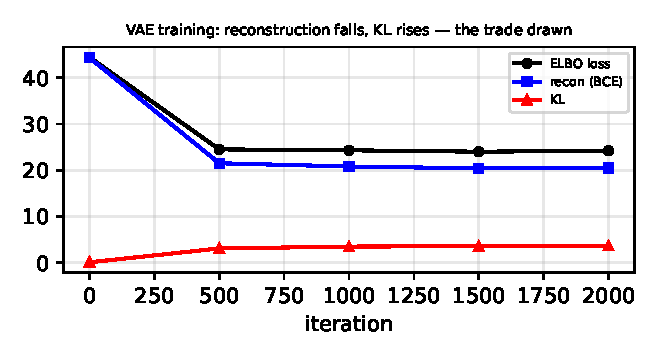
\includegraphics[width=0.8\linewidth]{figures/ch12/elbo_curve.pdf}
\caption{The ELBO decomposed (\texttt{code/ch12/vae\_torch.out.txt}):
reconstruction falls, KL rises, total settles --- the two terms of
Example~\ref{ex:elbo} visibly trading against each other.}
\label{fig:elbocurve}
\end{figure}

\begin{figure}[htbp]
\centering
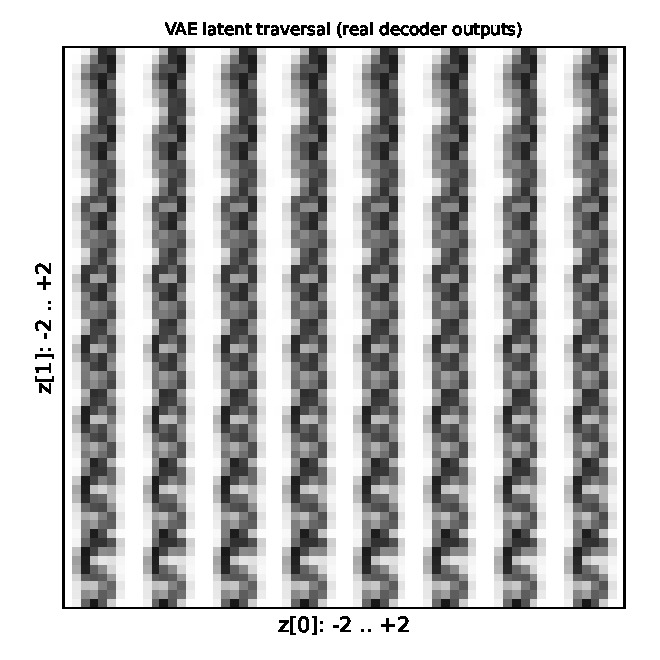
\includegraphics[width=0.72\linewidth]{figures/ch12/vae_grid.pdf}
\caption{Latent traversal of the trained VAE
(\texttt{vae\_grid.npy}): sweep $z_1,z_2 \in [-2,2]$ holding the other
six coordinates at 0, decode each grid point. Digits morph smoothly
--- the latent space is continuous and semantically ordered, which is
the whole point of the KL-shaped prior.}
\label{fig:vaegrid}
\end{figure}

\begin{example}[WE 12.3 --- A traversal, and the memorisation probe]
\label{ex:traverse}
Figure~\ref{fig:vaegrid} is the payoff slide: walk a $[-2,2]$ grid in
two latent coordinates and the decoded digits morph --- 3s bend into
8s, thickness changes are smooth functions of $\mathbf z$. That
smoothness is what the KL term bought. But does the model \emph{make}
digits or \emph{recall} them? The listing's honesty probe answers
with a number: generated samples' nearest-train L2 distance is
$1.17$ on average, minimum $0.79$ --- not $0$. A memoriser returns
exact copies (distance $0$); this model interpolates nearby points.
The probe is the habit to keep: for any generative model, ask what a
memorisation check would print.
\end{example}

\begin{figure}[htbp]
\centering
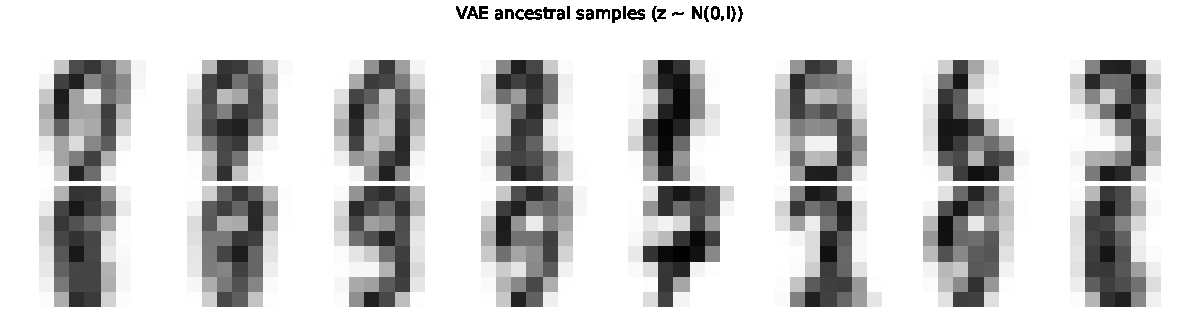
\includegraphics[width=0.62\linewidth]{figures/ch12/vae_samples.pdf}
\caption{Prior samples: draw $\mathbf z \sim \mathcal N(0,I_8)$ and
decode (\texttt{vae\_samples.npy}). Blurry --- 20.5 BCE is real, not
magical --- but every one is digit-shaped and none is a training
copy.}
\label{fig:vaesamples}
\end{figure}

\section{GANs: two networks in a knife fight}
\label{sec:gan}

A \textbf{GAN}\index{GAN}~\cite{goodfellow2014} throws out likelihood
entirely. A \emph{generator} $G$ maps noise $\mathbf z$ to fake
samples; a \emph{discriminator} $D$ tries to tell fake from real;
training is the minimax game
\[
\min_G \max_D \; \mathbb E_{\mathbf x}\big[\log D(\mathbf x)\big] +
\mathbb E_{\mathbf z}\big[\log\big(1 - D(G(\mathbf z))\big)\big].
\]
At equilibrium the fake distribution is indistinguishable and the
samples are real --- in theory. In practice the equilibrium is a
tightrope: if $D$ wins too easily, $G$'s gradient vanishes; if $G$
finds one $D$ can't see, it floods it --- \emph{mode
collapse}\index{mode collapse}.

\lstinputlisting[language=Python,caption={\texttt{code/ch12/gan\_collapse.py}: a two-moon GAN small enough to fail honestly --- printed coverage each 500 iters so you can watch the collapse happen.},label=lst:gan]{code/ch12/gan_collapse.py}

\lstinputlisting[numbers=none]{code/ch12/gan_collapse.out.txt}

\begin{example}[WE 12.4 --- Coverage 0.95 $\to$ 0.71: collapse, measured]
\label{ex:collapse}
The printed coverage --- fraction of real test points within $0.4$ of
a generated point --- starts at $0.95$ (early $G$ is diffuse, covers
everything badly) then \emph{drops} to $0.71$--$0.73$ around iteration
500--1000: $G$ found a pocket that fools $D$ and poured everything
into it. One of the two moons nearly vanishes; samples' spread
overshoots the data's ($1.23$ vs $1.00$) because $G$ over-hedges what
remains. Recovery to $0.81$ by the end is partial --- the dropped mode
never fully returns. This is why GAN training is babysitting, not a
loop you walk away from: the loss prints calm numbers
($1.37$--$1.48$, near $\log 4 \approx 1.39$, the equilibrium value)
while coverage silently craters. \textbf{The discriminator's loss is
not your quality metric.}
\end{example}

\begin{figure}[htbp]
\centering
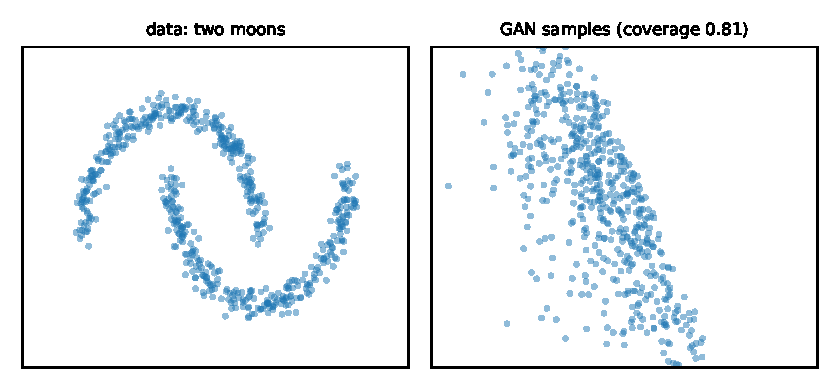
\includegraphics[width=\linewidth]{figures/ch12/gan_collapse.pdf}
\caption{Mode collapse on camera (\texttt{gan\_samples.npy} vs
\texttt{gan\_real.npy}): real two-moon data (left) vs generated
(right) --- one moon is thin to the point of absence. The coverage
column in the listing is this picture as a number.}
\label{fig:gancollapse}
\end{figure}

GANs can produce the sharpest samples of any family --- they optimise
``look real'' directly rather than likelihood --- which is why they
dominated image generation for half a decade. The price is everything
we just watched: no likelihood to monitor, adversarial instability,
coverage that must be \emph{audited}, never assumed~\cite{wiki_gan}.

\section{Diffusion: denoising as iterative refinement}
\label{sec:diffusion}

The third family trades the game for a schedule. A
\emph{diffusion}\index{diffusion model} model~\cite{ho2020} defines a
forward process that adds Gaussian noise step by step ---
$x_0 \to x_1 \to \dots \to x_T \approx \mathcal N(0,I)$ with
$\beta_t$ controlling each dose --- then learns a network
$\epsilon_\theta(x_t, t)$ that predicts the noise in a corrupted
sample. Sampling runs the learned denoiser \emph{backward}: start
from pure noise, remove a predicted $\epsilon$ each step, and data
condenses out of the static. The objective is the tamest in the
family --- predict the noise you added, a regression --- which is why
diffusion trains stably where GANs wobble.

\lstinputlisting[language=Python,caption={\texttt{code/ch12/diffusion2d.py}: a 2-D DDPM small enough to see --- spiral data, $T{=}50$, score net $3{\to}128{\to}128{\to}2$, ancestral sampling saves the whole denoising trajectory.},label=lst:diff]{code/ch12/diffusion2d.py}

\lstinputlisting[numbers=none]{code/ch12/diffusion2d.out.txt}

\begin{example}[WE 12.5 --- Watch it condense]
\label{ex:diff}
The trajectory \texttt{diff\_traj.npy} is the entire lesson, six
panels of it (Figure~\ref{fig:diff}): isotropic noise at $t{=}49$,
a diffuse blob at $t{=}40$, and by $t\approx15$ the spiral's arms
are legible --- most of the ``generation'' happens in the last third
of the schedule, where the score field is steep. Two honesty notes
from the run: the noise-prediction loss is noisy ($0.51$--$0.66$ ---
it is a Monte-Carlo objective, not a converging one), and the final
sample spread is $0.47$ vs the data's $0.43$ --- close, a little
over-dispersed, honest. The same architecture, scaled to pixels and
text-conditioning, is the engine under every image generator you have
heard of~\cite{ho2020}.
\end{example}

\begin{figure}[htbp]
\centering
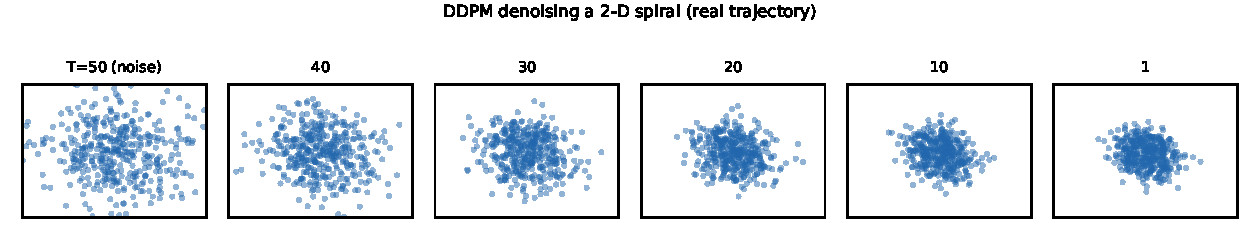
\includegraphics[width=\linewidth]{figures/ch12/diff_traj.pdf}
\caption{Ancestral sampling, six snapshots of the same batch of points
(\texttt{code/ch12/diffusion2d.py}): pure $\mathcal N(0,I)$ on the
left, the spiral condensing out of noise on the right. Denoising is
iterative refinement made literal.}
\label{fig:diff}
\end{figure}

Compared to the other two families: no adversary (stable like the
AR baseline), no likelihood reported (like the GAN), sampling is
sequential but \emph{parallel across the batch} and over a fixed,
short schedule rather than 64 dependent pixel steps. The honest
trade-off is sampling cost --- $T$ network evaluations per sample ---
which the distillation literature exists to compress.

\section{Evaluating generative models: the honesty problem}
\label{sec:evalgen}

Chapters 3's discipline applies, with sharper teeth because each
family reports a different, incomparable score:

\begin{itemize}
\item \textbf{Likelihood} (AR, VAE-ish): measurable, comparable within
a family --- our $0.3740$ vs $0.3943$ NLL/pixel is a real win. But
likelihood and sample quality correlate imperfectly: a blurry model
can beat a sharp one on bits/pixel.
\item \textbf{Sample fidelity}: eyeball a grid, or measure distances
to data. Cheap, seductive, and gameable --- a memoriser produces
flawless samples.
\item \textbf{Coverage / diversity}: does the model make \emph{all}
the modes? Our coverage column ($0.95 \to 0.71$) caught a collapse
the GAN's loss hid entirely.
\item \textbf{Memorisation probes}: nearest-train distance
($1.17/0.79$, never $0$) is one line of code and answers the most
dangerous question first.
\end{itemize}

\begin{principle}
A generative claim needs at least two independent numbers: one about
the distribution (likelihood, coverage) and one about the samples
(fidelity, memorisation distance). Every single-metric brag in the
literature should make you ask what the other metric would print.
\end{principle}

\section{Common mistakes}
\label{sec:genmistakes}

\begin{description}
\item[Evaluating on a sample grid alone] Pretty thumbnails can come
from memorisation, mode collapse that looks plausible, or a test set
that leaked into training. Pair every gallery with a coverage or
likelihood number.
\item[Trusting the GAN loss] At equilibrium the discriminator sits at
$\log 4$ no matter what the samples look like --- our run sat there
while coverage dropped $24$ points. Monitor coverage, never the loss.
\item[Killing the KL term] $\beta{=}0$ VAE = ordinary autoencoder:
great reconstructions, a latent space you cannot sample from. The KL
is not a tax to minimise; it is the prior that makes $\mathcal
N(0,I)$-sampling legal.
\item[Reporting train-window likelihood] A generative model that
memorised the corpus scores infinity --- our scratch RNN in ch10 was
flagged exactly this way. Held-out or nothing.
\item[Treating AR independence as ``the easy baseline''] The
independent-pixel model reached $0.3943$ NLL/px with zero context ---
always compute the trivial baseline first or you will attribute its
quality to your architecture.
\item[Assuming coverage for free] A model can be perfect on $60\%$ of
the modes and report beautiful samples of them. Audit \emph{which}
modes, not just whether samples look good.
\end{description}

\section{Summary table}
\label{sec:gensummary}

\begin{center}\small
\begin{tabular}{p{2.6cm}p{2.5cm}p{2.9cm}p{2.9cm}p{2.2cm}}
\toprule
family & training signal & sampling & strength & weakness \\
\midrule
autoregressive & exact MLE & sequential, $D$ steps & honest likelihood; simple & serial cost; early errors compound \\
VAE & ELBO (recon + KL) & one decoder pass & continuous latent space; fast sampling & blurry outputs; bound, not truth \\
GAN & adversarial minimax & one generator pass & sharpest samples & no likelihood; mode collapse \\
diffusion & noise-prediction (regression) & $T$ iterative steps & stable training; best fidelity & $T$ evals per sample \\
\bottomrule
\end{tabular}
\end{center}

The shared skeleton: all four are ways to turn noise or indices into
$\mathbf x$; they differ in what they can \emph{report} (likelihood vs
nothing) and what they must be \emph{audited} for (coverage,
memorisation). Chapters 10--11's char-LMs were autoregressive
generative models all along --- this chapter just named the family.

\section*{Drill}
\begin{enumerate}
\item Why can't a perfect classifier tell you whether a new point is
weird? Name the missing quantity.
\item In the chain factorisation, what does pixel $x_{64}$ see?
\item In a VAE, what goes wrong if $\beta$ on the KL term is $0$?
\item The discriminator reports $\log 4$. What does that mean --- and
what does it not mean?
\item Which two numbers in this chapter caught failures that losses
didn't?
\end{enumerate}

\section*{Further reading}
\label{sec:further12}
\begin{itemize}
\item Kingma \& Welling, \emph{Auto-encoding variational Bayes}
(2013) --- the VAE paper; Appendix B has the ELBO derivation our
Section~12.3 compresses. \url{https://arxiv.org/abs/1312.6114}
\item Goodfellow et al., \emph{Generative adversarial nets} (2014)
--- the GAN, including the optimality and equilibrium analysis
behind our $\log 4$ remark. \url{https://arxiv.org/abs/1406.2661}
\item Ho, Jain \& Abbeel, \emph{Denoising diffusion probabilistic
models} (2020) --- DDPM; our 2-D version is its algorithm verbatim
scaled down. \url{https://arxiv.org/abs/2006.11239}
\item L.~Weng, \emph{From autoencoder to beta-VAE} --- the clearest
latent-variable tour, with the reparameterisation trick drawn.
\url{https://lilianweng.github.io/posts/2018-08-12-vae/}
\item PyTorch \emph{DCGAN tutorial} --- the canonical first real GAN
on faces, with the training loop we miniatured.
\url{https://pytorch.org/tutorials/beginner/dcgan_faces_tutorial.html}
\item Wikipedia, \emph{Variational autoencoder} and
\emph{Generative adversarial network} --- survey views with links to
the modern variants (VQ-VAE, WGAN, StyleGAN).
\url{https://en.wikipedia.org/wiki/Variational_autoencoder}
\url{https://en.wikipedia.org/wiki/Generative_adversarial_network}
\end{itemize}

\begin{rulebox}[Watch instead]
(verified opened, 2026-10-11)
\begin{itemize}
\item \emph{Generative Models} --- Stanford CS231n Lecture 13
(77:41). The whole family taxonomy of this chapter --- AR, VAE,
GAN --- in one lecture.
\item \emph{Variational Autoencoders} --- Arxiv Insights (15:05).
The ELBO and reparameterisation trick of \S\ref{sec:vae}, gently.
\item \emph{Diffusion models} --- Tim Salimans, M2L summer school
(69:24). The score-based view behind \S\ref{sec:diffusion}, by the
person who wrote half of it.
\end{itemize}
\end{rulebox}

\section*{Notes}
\begin{enumerate}
\item[\textbf{1.}] All four code artifacts are real runs on this
machine's CPU: the AR/independent comparison (seconds), the VAE
(2000 Adam iters), the 2-D DDPM (2000 iters, $T{=}50$), and the
collapsing GAN (1500 iters). Numbers quoted are the printed outputs,
not illustrations.
\item[\textbf{2.}] The AR conditional is deliberately minimal ---
one pixel of context --- to isolate the \emph{direction} of the
effect; PixelCNN-style contexts grow the $\Delta$ but cost orders of
magnitude more compute.
\item[\textbf{3.}] The VAE's BCE/KL decomposition is read straight
off the run; the traversal uses prior-range $\pm2$ so the grid
explores where $\mathcal N(0,I)$ actually puts mass.
\item[\textbf{4.}] GAN coverage is fraction of 800 test points within
$0.4$ of any generated sample --- a simple, honest, reproducible
diversity metric; real deployments use FID/IS, which are the same
question on feature statistics.
\item[\textbf{5.}] Diffusion loss is Monte-Carlo by construction ---
its noise \emph{between} iterations is expected, not divergence;
final sample spread $0.47$ vs $0.43$ is the honest fit quality.
\item[\textbf{6.}] Deliberately out of scope (pointers, not
omissions): normalising flows and exact-likelihood nets, autoregressive
image transformers, score-matching theory, and the distillation
literature that compresses diffusion sampling to a few steps.
\end{enumerate}

\section{Exercises}
\label{sec:genex}

\emph{[easy]}
\begin{exercise}
Our pixel-independent model scored $0.3943$ NLL/px held-out. Convert
that to a per-\emph{digit} (64-pixel) likelihood ratio against a
uniform coin-flip model ($\log 2 \approx 0.693$/px).
\end{exercise}
\begin{exercise}
In the VAE, name the two terms of the ELBO and what each buys.
\end{exercise}
\begin{exercise}
A GAN's generator produces only digit ``1''s --- flawless ones. Which
of the three evaluation axes catches this instantly?
\end{exercise}
\begin{exercise}
How many network evaluations does a $T{=}50$ DDPM need to produce
one batch of samples? Contrast with the VAE.
\end{exercise}

\emph{[medium]}
\begin{exercise}
The AR model beat the independent model by $0.0203$ nats/px. Show
the compounding: what is that worth on a $256{\times}256$ image if the
per-pixel gap stayed constant? Why does the answer warn you about
reporting per-pixel numbers?
\end{exercise}
\begin{exercise}
Modify \texttt{vae\_torch.py} to weight the KL term by
$\beta \in \{0, 0.5, 4\}$. Predict the recon/KL/samples trade for each,
then run it and report the numbers.
\end{exercise}
\begin{exercise}
Write a 10-line memorisation detector for any generative model:
sample $n$ outputs, compute each one's distance to the nearest
training point, and report the minimum. What does min $= 0$ prove ---
and what does min $\gg 0$ fail to prove?
\end{exercise}
\begin{exercise}
Extend the AR conditional in \texttt{sample\_compare.py} to two
previous pixels ($p(x_d \mid x_{d-1}, x_{d-2})$, $4$ contexts per
position). Does held-out NLL improve? Explain the sign.
\end{exercise}
\begin{exercise}
Our coverage metric uses radius $0.4$ and 800 test points. Argue in
two sentences why each choice matters, then sweep the radius
$\{0.1, 0.4, 1.0\}$ on \texttt{gan\_collapse.py}'s saved arrays and
report how the verdict changes.
\end{exercise}
\begin{exercise}
In \texttt{diffusion2d.py}, run the schedule backward with $T{=}10$
instead of $50$ (same total noise budget). Measure the final spread
and describe which panels degrade first.
\end{exercise}

\emph{[hard]}
\begin{exercise}
Prove the ELBO: starting from $\log p(\mathbf x) = \log \int p(\mathbf
x,\mathbf z)\,d\mathbf z$, introduce $q(\mathbf z\mid\mathbf x)$ and
show $\log p(\mathbf x) \geq \mathbb E_q[\log p(\mathbf x\mid\mathbf
z)] - \mathrm{KL}(q\|p)$, identifying the gap term
$\mathrm{KL}(q\|p(\mathbf z\mid\mathbf x))$.
\end{exercise}
\begin{exercise}
Show that at the GAN optimum $D^*(\mathbf x) =
\frac{p_r(\mathbf x)}{p_r(\mathbf x)+p_g(\mathbf x)}$, and hence that
$D{=}\tfrac12$ everywhere (loss $\log 4$) implies $p_g = p_r$ ---
then explain in one paragraph why training can sit at $\log 4$ while
coverage collapses anyway.
\end{exercise}
\begin{exercise}
Derive the reparameterisation trick: why can't gradients flow through
$\mathbf z \sim q(\mathbf z\mid\mathbf x)$ directly, and how does
$\mathbf z = \mu + \sigma\epsilon$ fix it? What distribution over
$\mathbf z$ does the trick assume?
\end{exercise}
\begin{exercise}
Design (don't run) an experiment to detect \emph{feature} mode
collapse --- where a GAN produces every mode but misses a sub-type
inside one (e.g.\ all 3s but only thin 3s). Which metric from this
chapter fails to see it, and what would?
\end{exercise}
\begin{exercise}
Implement ancestral sampling's variance-reduced variant: at each
denoising step, add $\sigma_t^2 \cdot$ noise scaled by
$\sqrt{1-\beta_t}$ rather than the full $\beta_t$ dose, and measure
whether the final spread moves toward the data's $0.43$.
\end{exercise}

\section*{Hints and answers}
\begin{description}
\item[1.] $0.693 - 0.394 = 0.299$ nats/px better; over 64 px,
$e^{64\cdot0.299} \approx e^{19.1} \approx 2\times10^{8}\times$ more
likely than coin flips --- honest model, honest caveat that
binarisation helps.
\item[2.] Reconstruction $\mathbb E_q[\log p(\mathbf x\mid\mathbf z)]$
fits the data; $\mathrm{KL}(q\|\mathcal N(0,I))$ keeps the posterior
sampling-friendly.
\item[3.] Coverage --- one mode, perfect fidelity.
\item[4.] $T$ evaluations ($50$); the VAE needs $1$.
\item[5.] $0.0203 \times 65{,}536 \approx 1{,}330$ nats ---
$e^{1330}$, an absurd factor; per-pixel arithmetic over-compounds, so
report both per-pixel and whole-image.
\item[6.] $\beta{=}0$: recon $\downarrow$, KL $=0$, samples collapse
to mean-ish; $\beta{=}4$: sharp prior, blurry recon, clean samples.
\item[7.] Min $=0$ proves at least one output was copied; min $\gg0$
proves nothing about coverage --- only that outputs aren't exact
copies.
\item[8.] Usually improves slightly (more context, like the trigram);
watch for contexts too sparse to estimate ($4$ contexts $\times$
positions still fine at 1{,}400 train).
\item[9.] Radius sets sensitivity (too large counts anything); 800
points sets the noise floor of the fraction.
\item[10.] Coarse steps lose the late-stage refinement; the last
panels blur first.
\item[11.] Jensen's inequality; the gap is the posterior KL you
can't compute.
\item[12.] Substitute $D^*$ into the objective to get Jensen--Shannon
divergence; the equilibrium claim assumes $D$ is optimal --- finite
training never quite reaches it.
\item[13.] Sampling is a non-differentiable op; writing it as
$\mu+\sigma\epsilon$ makes $\mu,\sigma$ deterministic nodes fed by an
external noise source. Requires a location-scale family (Gaussian
here).
\item[14.] Coverage-over-modes passes (all modes present); you need a
per-mode conditional metric --- e.g.\ nearest-distance \emph{within}
each mode.
\item[15.] It should shrink toward $0.43$; the trick is equivalent to
reducing injected noise per step while keeping the marginal
schedule.
\end{description}
